\documentclass[12pt]{article}
%\usepackage{graphicx}
\usepackage{indentfirst}
\usepackage[export]{adjustbox}
\usepackage{graphicx}
\usepackage{float}
\usepackage{hyperref}

%opening
\title{Audio effects library\\Overall description of project}
\author{Kacper Harezga\\Ewa Kobiela\\Jan Laskowski\\Krzysztof Sobczyk\\Grzegorz Machura}
\date{10.04.2021}
\begin{document}
	
	\maketitle
	\tableofcontents
	\newpage

\section{Project charter}

	\begin{figure}[H]
		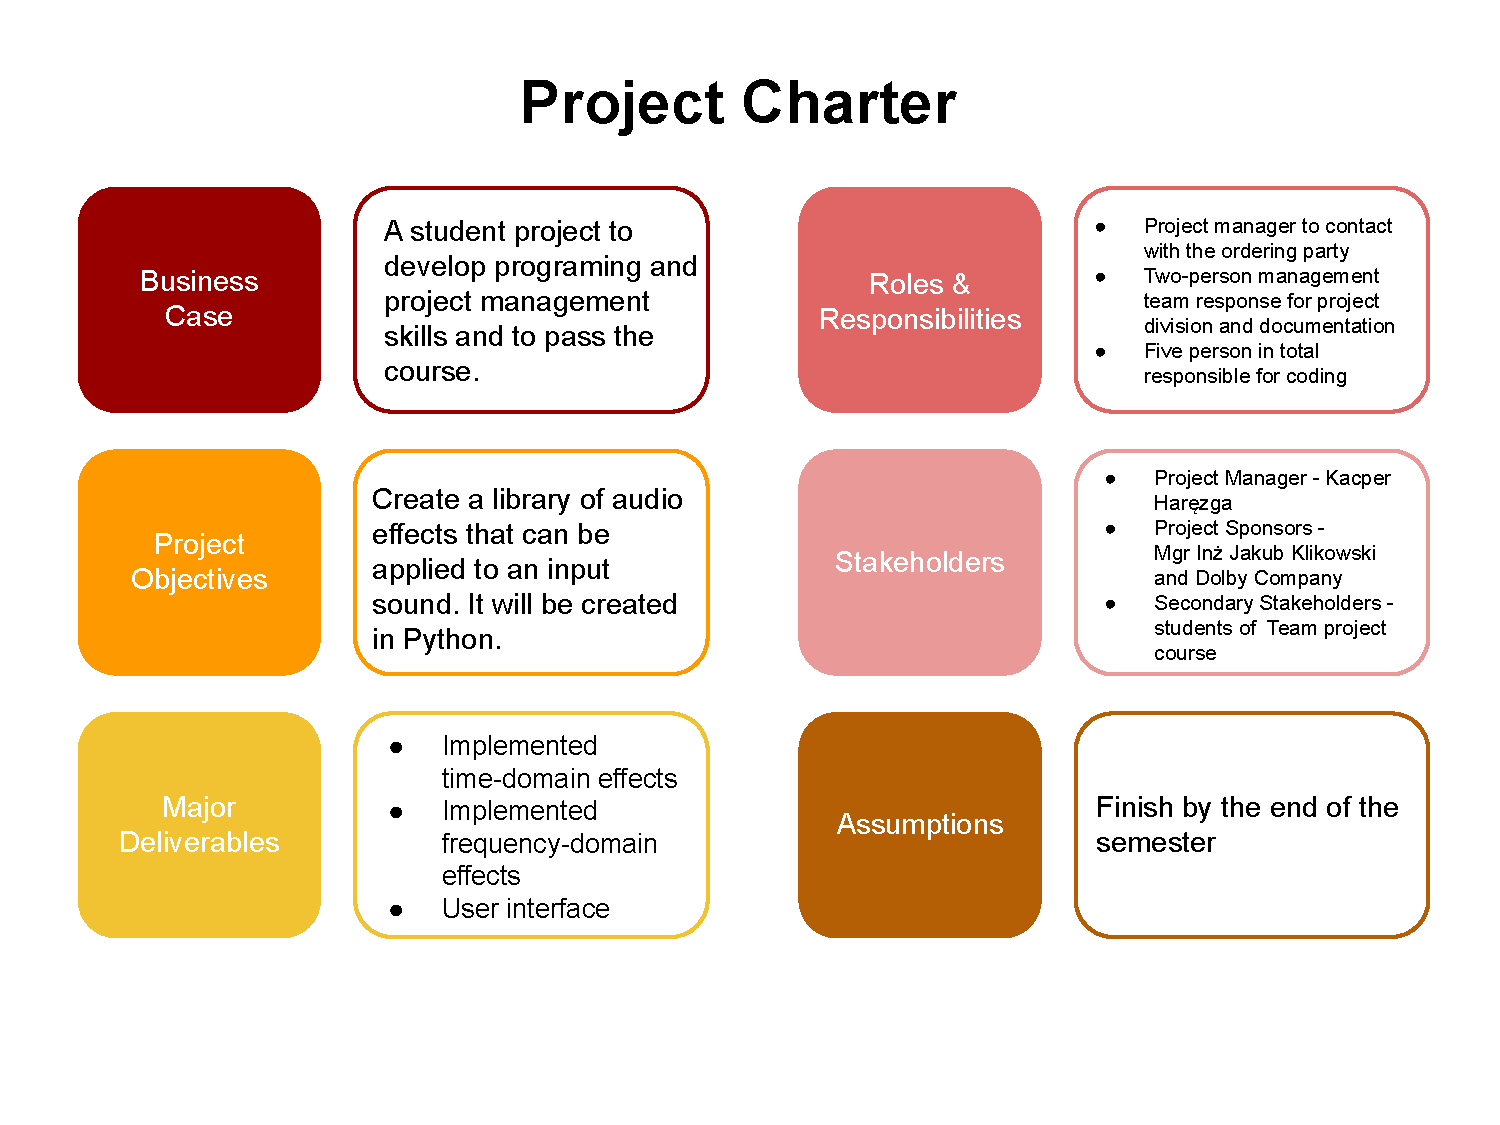
\includegraphics[width=1.2\textwidth, center]{Project charter}
	\end{figure}
	

\section{Topic of the project}

	\begin{figure}[H]
		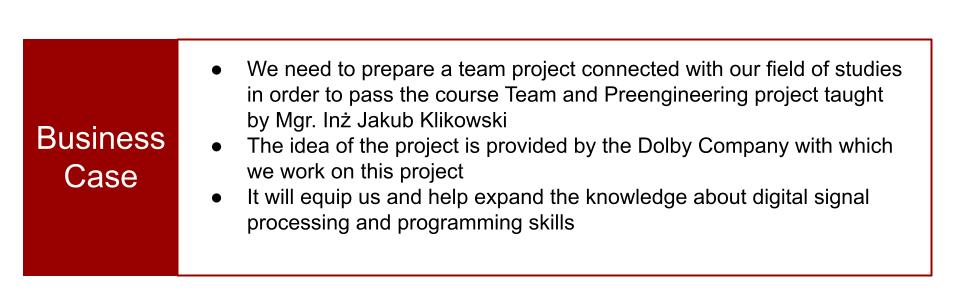
\includegraphics[width=1.2\textwidth, center]{Business Case}
	\end{figure}

The goal of this project is to create a library of real-time audio effects. It will consist several types of audio effects, including delay/echo, FIR, compressor, band equalizer, pitch shifter etc. I will allow to process any unrestricted input signal into a desired output with a chosen type of filtering. We will be using a wide range of processors in order to create different audio effect, operating on both frequency and time domain.

The architecture of the project will consist of a library of functions performing applied audio effects. We will also implement a part of application that will allow user to process chosen audio file with one of implemented effects. Moreover, for the presentation of our results, we will create a demo showing abilities of our application.

\section{The purpose of the project}

	\begin{figure}[H]
		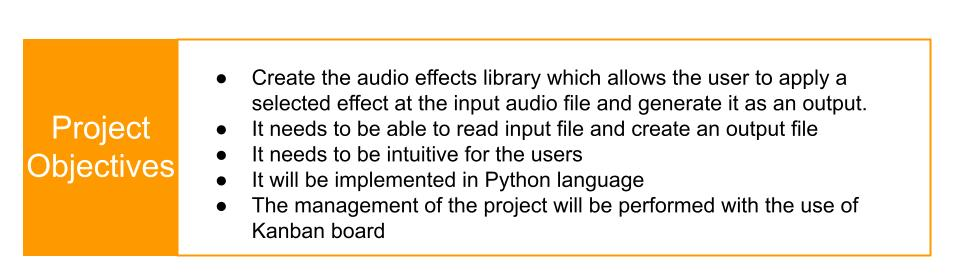
\includegraphics[width=1.2\textwidth, center]{Project Objectives}
	\end{figure}
	
	\begin{figure}[H]
		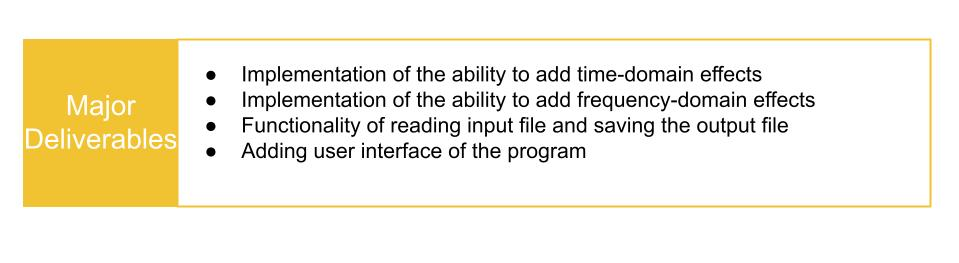
\includegraphics[width=1.2\textwidth, center]{Major Deliverables}
	\end{figure}
	
	\begin{figure}[H]
		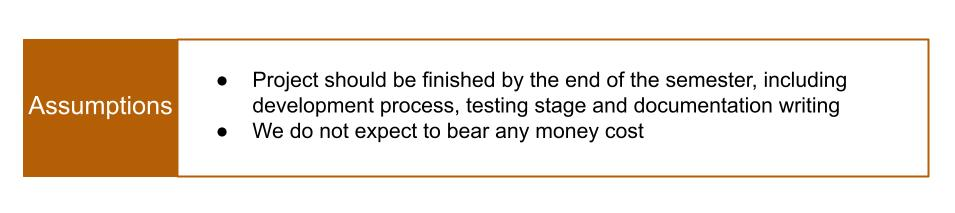
\includegraphics[width=1.2\textwidth, center]{Assumptions}
	\end{figure}

The Audio effects library and application is requested by the client, which is  Dolby Laboratories, Inc. The topic was presented on the Team Project Conference as an opportunity for students not only to learn about digital signal processing and practice or expand programming skills, but additionally to get familiar with cooperation for a professional company and gain experience with working on a client requesting solution with given requirements.

Dolby Laboratories, Inc. produces various audio devices, such as speakers, headphones and audio systems. The audio effects library can be used in those systems or devices in the process of correcting input sound to met the desired quality, feelings and to improve performance in objects with low acoustic infrastructure.

Moreover, the library might be used by amateurs, people interested in creating music or sound samples, by assisting them in obtaining the desired audio effects. If could also be implemented in home or car hi-fi sets as a additional method to improve the sound quality.

\section{Group composition}

	\begin{figure}[H]
		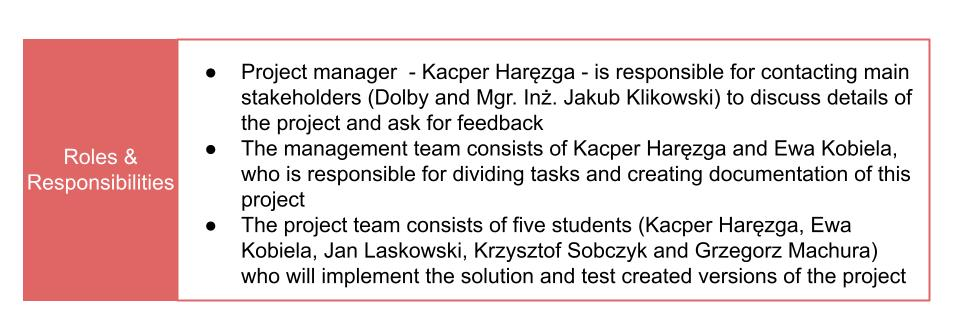
\includegraphics[width=1.2\textwidth, center]{Roles & Responsibilities}
	\end{figure}

The project group consists of five students: Kacper Harezga, Ewa Kobiela, Jan Laskowski, Krzysztof Sobczyk and Grzegorz Machura. Tasks are divided among project members equally based on individual predispositions. Although, the group chosen Kacper Harezga as a representative person for contacts with a client company. The rest of a group will be focused on researching, developing and testing solutions and writing project documentation.

\section{The stakeholders}

	\begin{figure}[H]
		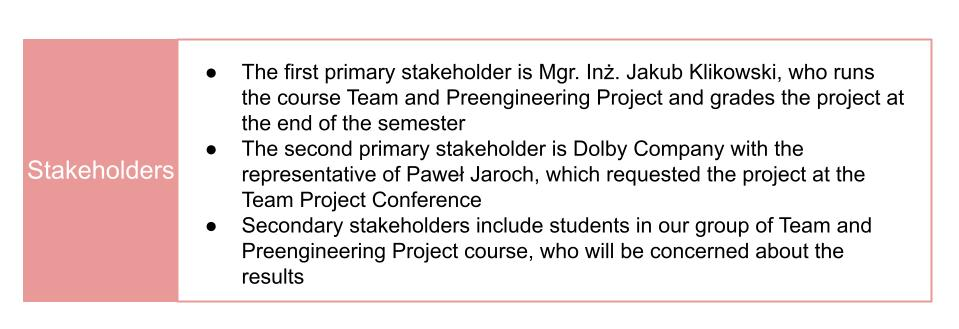
\includegraphics[width=1.2\textwidth, center]{Stakeholders}
	\end{figure}

The client for this application which proposed the topic and form of the project is the Dolby Laboratories, Inc. The company was the part who defined technology that will be used during development of the application. The company also committed to provide the necessary knowledge for the team needed to process signals and to assure, that the product will be suitable to be applied in bigger audio systems.

The hands-on users of the product were defined as engineers from Dolby Laboratories Inc. working on improvement on current audio solutions or creating new sound hardware. We assume that the user would have at least a basic knowledge about signal processing and our system would be a tool that they would use and implement in their work. In order to use our product, they would need to provide their own sound inputs and be aware of characteristics of each of implemented type of filters.

\subsection{Personas}

An example user, Bob is a young music enthusiast. He enjoys playing electrical guitar and is practising to raise his skills to the next level. He would like to add an echo effect to recording of a song he played in order to make it sound deeper and send the demo to a recording company. He would buy a plug-in to his favourite sound editing software from Dolby Laboratories Inc., that would consist of Audio Effects Library which allows them to add desired echo effect to his recording.


\end{document}
